\section*{Problem 2}

For the following system:
\begin{enumerate}
\item Find the first 6 values for the impulse input $x[n]=\delta_0$
\item Find the first 6 values for the unitary step input $x[n]=u[n]$
\item Find the analytical expression for the system
\end{enumerate} 

\begin{figure}[H]
\caption*{}
\centering
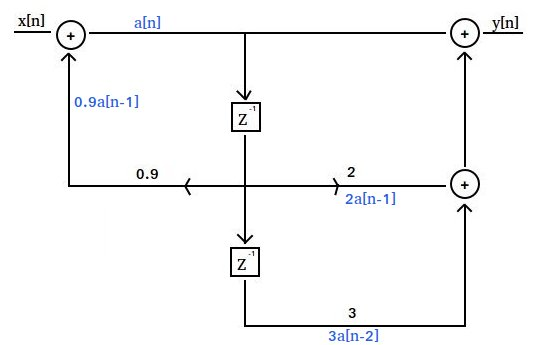
\includegraphics[width=0.8\textwidth]{figs/c7p2.jpg}
\label{fig:c7p2}
\end{figure} 

\subsection*{Solution}
From the follwing code (in C++) we get the first 6 values of the system
for the 2 proposed inputs:
\zcodec{../ztransform/c7p6.cpp}{C++ Implementation}

\begin{enumerate}
\setcounter{enumi}{0}
\item First 6 values of the system for the impulse input:
\begin{verbatim}
y[0] = 1.00000
y[1] = 2.90000
y[2] = 5.61000
y[3] = 5.04900
y[4] = 4.54410
y[5] = 4.08969
\end{verbatim}
\end{enumerate} 

\begin{enumerate}
\setcounter{enumi}{1}
\item First 6 values of the system for the unitary step input:
\begin{verbatim}
y[0] = 1.00000
y[1] = 3.90000
y[2] = 9.51000
y[3] = 14.55900
y[4] = 19.10310
y[5] = 23.19279
\end{verbatim}
\end{enumerate} 

\begin{enumerate}
\setcounter{enumi}{2}
\item Analytical expression:
\end{enumerate} 

\begin{equation*}
\begin{aligned}
y[n] &= a[n] + 2a[n-1] + 3a[n-2] \\
a[n] &= x[n] + 0.9a[n-1]
\end{aligned}
\end{equation*} 

Let $a[-1]=a[-2]=0$, then:

\begin{equation}
\begin{aligned}
a[z] + 2z^{-1}a[z]+3z^{-2}a[z] &= y[z] \\
z^{-2}a[z](z^2+2z+3] &= y[z]
\end{aligned}
\label{eq:c7p21}
\end{equation} 

and

\begin{equation}
\begin{aligned}
a[z] - 0.9z^{-1}a[z] &= x[z]\\
z^{-1}a[z](z-0.9z) &= x[z] \\
a[z] = \frac{x[z]}{z^{-1}(z-0.9)}
\end{aligned}
\label{eq:c7p22}
\end{equation}

From (\ref{eq:c7p21})  and (\ref{eq:c7p22}) we have:

\begin{equation*}
\begin{aligned}
y[z] &= z^{-1}\frac{x[z]}{z-0.9} (z^2+2z+3)\\
\frac{y[z]}{z} &= \frac{(x^2+2z+3)x[z]}{z^2(z-0.9)} \\
&= \frac{A}{z} + \frac{B}{z^2} + \frac{C}{z-0.9}
\end{aligned}
\end{equation*} 

Solving with partial fractions we have:

\begin{equation*}
\begin{aligned}
C= 6.92\\
B= -3.33\\
Az(z-0.9) + B(z-0.9) + cz^2 = z^2+2z+3\\
(A+C) = 1 \\
A = -5.92
\end{aligned}
\end{equation*} 

Therefore:

\begin{equation*}
\begin{aligned}
y[z] &= -5.92 - \frac{3.33}{z} + 6.92 \frac{z}{z-0.9} \\
y[n] &= -5.92 \delta_0[n] - 3.33 \delta_0[n-1] + 6.92 (0.9)^n
\end{aligned}
\end{equation*} 

